%!TEX root = Pflichtenheft.tex

\section{Benutzeroberfläche}

\subsection{Kommando-Struktur}
Die Kommando-Struktur der Benutzeroberfläche ist durch das Programm \emph{git} inspiriert\\
\\\\
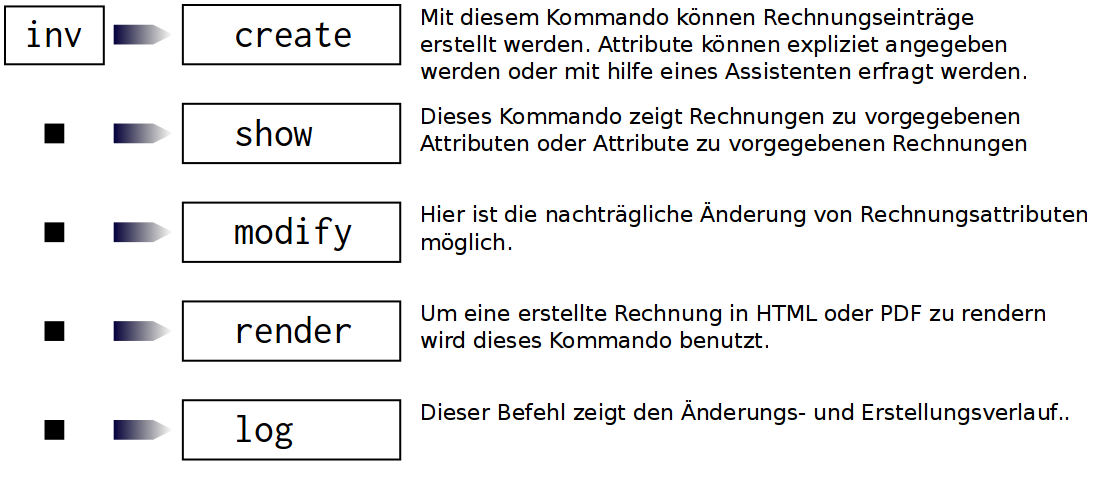
\includegraphics[width=\textwidth]{kommando-struktur.png}
\\
\subsection{Ordnerstruktur}
Es ist möglich mit der Ordnerstruktur innerhalb eines Repositories diverse
Standard-Attributwerte zu definieren. Dies geschieht im Zusammenhang mit den vom
Benutzer gewählten Ordnungsschlüsseln.\\
\\\\
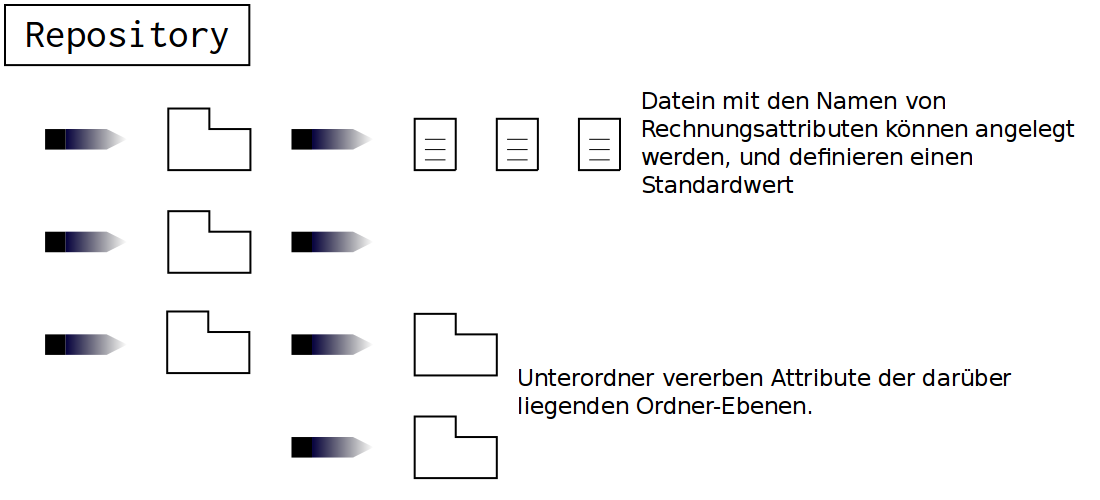
\includegraphics[width=\textwidth]{ordnerstruktur-struktur.png}
\\\\
\subsubsection*{Beispiel:}
Der Nutzer legt in seinem Rechnungsrepository jeweils einen Ordner für jeden Kunde
an. In jedem dieser Verzeichnisse plaziert er weiterhin eine Datei mit dem Namen
\emph{Adresse} worin er die Adresse des jeweiligen Kunden einträgt. Wenn er jetzt
im entsprechenden Kundenordner eine Rechnung kreiert ist das Attribut \emph{Adresse}
schon gesetzt.
